% Licensed to the Apache Software Foundation (ASF) under one or more
% contributor license agreements. See the NOTICE file distributed with
% this work for additional information regarding copyright ownership.
% The ASF licenses this file to You under the Apache License, Version 2.0
% (the ``License''); you may not use this file except in compliance with
% the License. You may obtain a copy of the License at
%
% http://www.apache.org/licenses/LICENSE-2.0
%
% Unless required by applicable law or agreed to in writing, software
% distributed under the License is distributed on an ``AS IS'' BASIS,
% WITHOUT WARRANTIES OR CONDITIONS OF ANY KIND, either express or implied.
% See the License for the specific language governing permissions and
% limitations under the License.

\subsubsection{Configuring a Livelink Repository}

You must fill in the following extra tabs if you are creating a
Livelink repository connection:

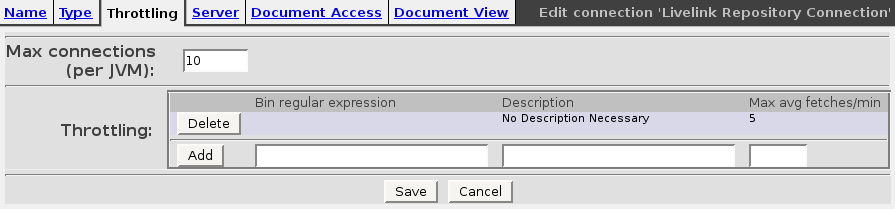
\includegraphics[width=300pt]{edit-repository-tab3}

\begin{itemize}

\item \textbf{Max connections (per JVM):} Here you can specify a
maximum number of connections for your repository. \ifCombinedConnectorGuide
The maximum number of connections per JVM is important for three
reasons; licensing, appliance resources, and the possiblity of
overwhelming the ingestion interface. For a more complete explanation,
see the Max Connections item on page \pageref{maxrepocon}.\fi

\ifLivelinkGuide
The maximum number of connections per JVM is important for three reasons.
First, the number of connections may impact the licensing on your document
server, depending on the repository. If you have a finite number of
Livelink connections available, they will be split between the authority
connector, which authorizes user access to documents, and the repository
connector, which actually downloads the documents to the appliance.

Second, the number of connections may impact the resources
available on the appliance. If the connector framework is slowing down
your appliance, lowering this number should help.

Third, only ten document streams can be processed by the appliance
at one time.  If you are also using other repository connectors or
the \command{ingest} command on the appliance, you should reduce this
number to prevent contention for the Ingestion interface. The Livelink
Connector will never overwhelm the interface on its own, but when other
applications are also using the ingestion interface, it may be best to
set the number of repository connections to five or even fewer.
\fi

\item \textbf{Throttling:} This allows you to set a maximum document
fetch rate from the repository.


The maximum fetch rate allows you to set three things: Expression,
description, and fetches per minute. Expression allows you to provide
a regular expression to match against document bins.  Each document
ingested through a connector is associated with one or more document
bins. These bins represent the servers that the connector interacts
with to obtain the document.  Typically, a document will be associated
with only one document bin, representing the repository server hosting
the document. For some repository connections, documents ingested
through the connector can be hosted by different servers. In the
Livelink Connector, documents only come from one server, which you
will set on the following tab. Simply leave the expression blank; this
will match any server you enter on the following tab.  All you need to
set is the number of document fetches per minute.  Description is an
optional field that allows you to provide a short text description of
the throttle.  Once you have set the fetch rate and optional
description, click Add.


\end{itemize}

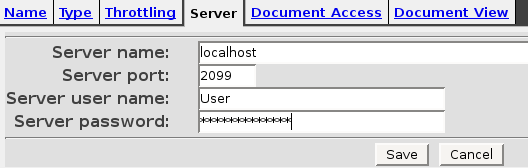
\includegraphics[width=300pt]{edit-repository-tab4}

\begin{itemize}

\item \textbf{Server name:} The name of the Livelink server from which you wish
to crawl documents.

\item \textbf{Server port:} The port on the Livelink server to which you
should connect. If you don't know what value this should be, ask your
Livelink administrator.

\item \textbf{Server user name:} The username you were given by your
Livelink administrator for connecting to the server. (The user account
must have sufficient authority to retrieve documents.)

\item \textbf{Server password:} The password you were given by your
Livelink administrator for the above username.

\end{itemize}

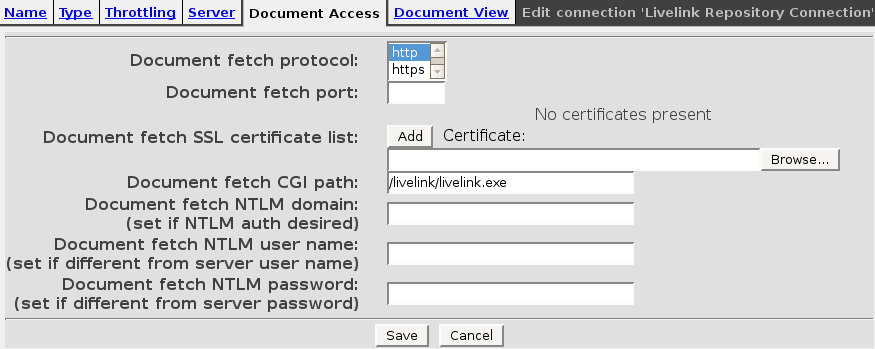
\includegraphics[width=300pt]{edit-repository-tab5}

These options all concern ``fetching'' documents, that is, the paths
that the Connector Framework should use when collecting documents for
ingestion to the MetaCarta search system. 

\begin{itemize}

\item \textbf{Document fetch protocol:} If you are connecting to an
open Livelink repository, choose ``http.'' If you are connecting using
SSL, choose ``https.''

\item \textbf{Document fetch port:} The port to use when connecting
to the Livelink server. If you are using the default port (80 for
http, 443 for https) you can leave this field blank. 

\item \textbf{Document fetch SSL certificate list:} Some Livelink servers
require that you authenticate via SSL before downloading documents. By
clicking the ``Browse'' button, you can select an SSL certificate that
the appliance should trust for authentication to the Livelink server. Clicking
``Add'' will upload the certificate to the appliance.

To get such a certificate, visit the Livelink repository from your
web browser and save the file, or ask your Livelink administrator.
For maximum robustness, you should add the certificate for the certificate
authority that signed the Livelink repository certificate rather than
the Livelink certificate itself. To do this, contact your site's security
administrators. In some cases, you may need more than one certificate.

\item \textbf{Document fetch CGI path:} The path on the Livelink server that the
appliance should use to crawl for documents.

\item \textbf{Document fetch NTLM domain:} The NTLM domain 
through which the crawler should access the Livelink repository, if required.

\item \textbf{Document fetch NTLM user name:} The user name to use for 
NTLM, if different from the user name used to connect to the server.

\item \textbf{Document fetch NTLM password:} The password to use for
NTLM, if different from the password used to connect to the server.

\end{itemize}

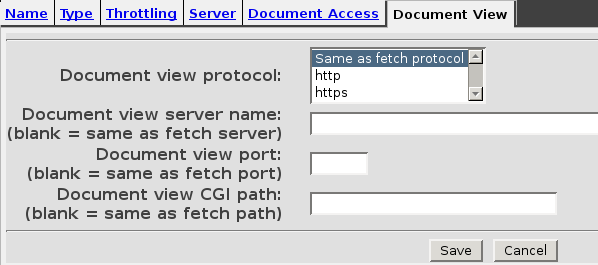
\includegraphics[width=300pt]{edit-repository-tab6}

These options all concern ``viewing'' documents, that is, the URLs
at which users are directed to documents when they see the documents
as search results. These options can be used to change the URLs of
documents crawled through Livelink before they are sent to the MetaCarta
Ingestion API. They do not change anything about the documents in the
Livelink repository itself. 

\begin{itemize}

\item \textbf{Document view protocol:} If end users are connecting to an open
Livelink repository, choose ``http.'' If users are connecting using SSL,
choose ``https.'' If users are connecting to the same Livelink instance
as the crawler, choose ``Same as fetch protocol.''

\item \textbf{Document view server:} The server to use when giving end
users links to a Livelink server as part of search results. If you
are using the same server as for document fetch, you can leave this
field blank.

\item \textbf{Document view port:} The port to use when giving end users
links to the Livelink server as part of search results. If you are using
the same port as for document fetch, you can leave this field blank.

\item \textbf{Document view CGI path:} The path on the Livelink server
that the end user should use when viewing document search results. This
is usually the same as the fetch path, but if it is not, you can set
it here. If this is different from the document fetch CGI path, it is
likely because the appliance has different permissions from normal users,
but it may also be because you want users to access a different Livelink
server from the appliance. This setting (along with the NTLM domain,
described above) determines the URL given to users of the Web Search
Interface, MetaCarta Search APIs, and the ESRI ArcMap Extension.

\end{itemize}


After entering this information, you will be taken to the repository 
connection status page for this repository:

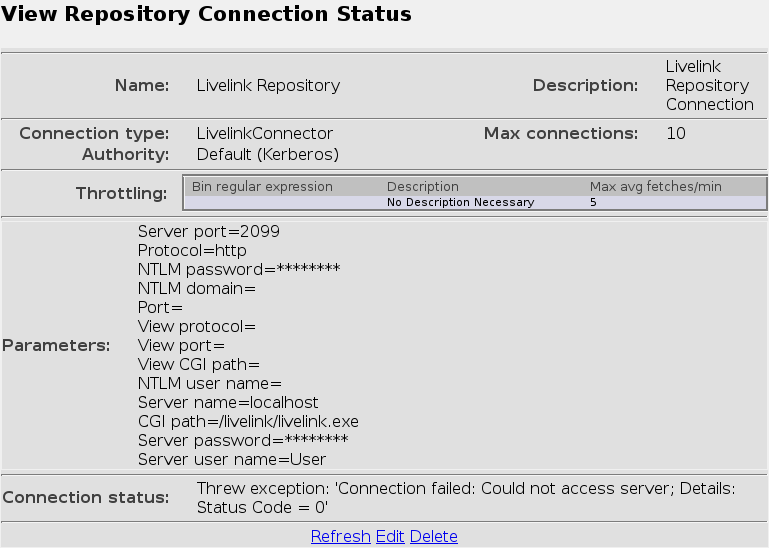
\includegraphics[width=300pt]{view-repo-conn-status}

In this example (which does not contain accurate information for any
Livelink server), the Connection Status is ``Connection failed.''
If you see this message, you most likely have incorrectly entered one
of the fields, and should click ``Edit'' to fix the data. If you have
entered everything as you intended, please inform your Livelink administrator;
you may not have been given the correct information.
